\documentclass[border=8pt,tikz]{standalone}
\usepackage{amsmath}
\usetikzlibrary{arrows.meta, fit, positioning, backgrounds}
\usepackage[outline]{contour}
\contourlength{1.4pt}

\usepackage{helvet}
\renewcommand{\familydefault}{\sfdefault}
\usepackage{sansmath}
\sansmath
\DeclareSymbolFont{sfoperators}{OML}{cmm}{m}{it}
\DeclareMathSymbol{\Delta}{\mathalpha}{sfoperators}{"01}

% COLORS
\usepackage{xcolor}
% UCL brand accessible data-viz palette (matches Neural_Networks/basic_CO2, shared_CO_CO2)
\definecolor{uclDarkPurple}{HTML}{361A54}
\definecolor{uclLightPink}{HTML}{E645AB}
\definecolor{uclLightOrange}{HTML}{E66C37}
\definecolor{uclLightGreen}{HTML}{1AAB40}
\definecolor{uclLightBlue}{HTML}{118DFF}
\definecolor{uclDarkRed}{HTML}{751441}

% STYLES
\tikzset{
  >=latex,
  level/.style={thick,circle,draw=uclDarkPurple,fill=uclDarkPurple!85!white,minimum size=16,inner sep=0},
  iso edge/.style={thick,uclLightPink,line width=1.4pt},
  j edge/.style={thick,uclLightOrange,line width=1.4pt},
  term box/.style={draw,thick,rounded corners=4pt,align=center,font=\small,inner sep=6pt},
  term box iso/.style={term box,draw=uclLightPink!60!black,fill=uclLightPink!12},
  term box j/.style={term box,draw=uclLightOrange!60!black,fill=uclLightOrange!15},
  sum node/.style={thick,circle,draw=uclDarkRed,fill=uclDarkRed!10,minimum size=26,font=\small},
  label/.style={font=\small,align=center},
  axislabel/.style={font=\footnotesize,align=center}
}

\begin{document}
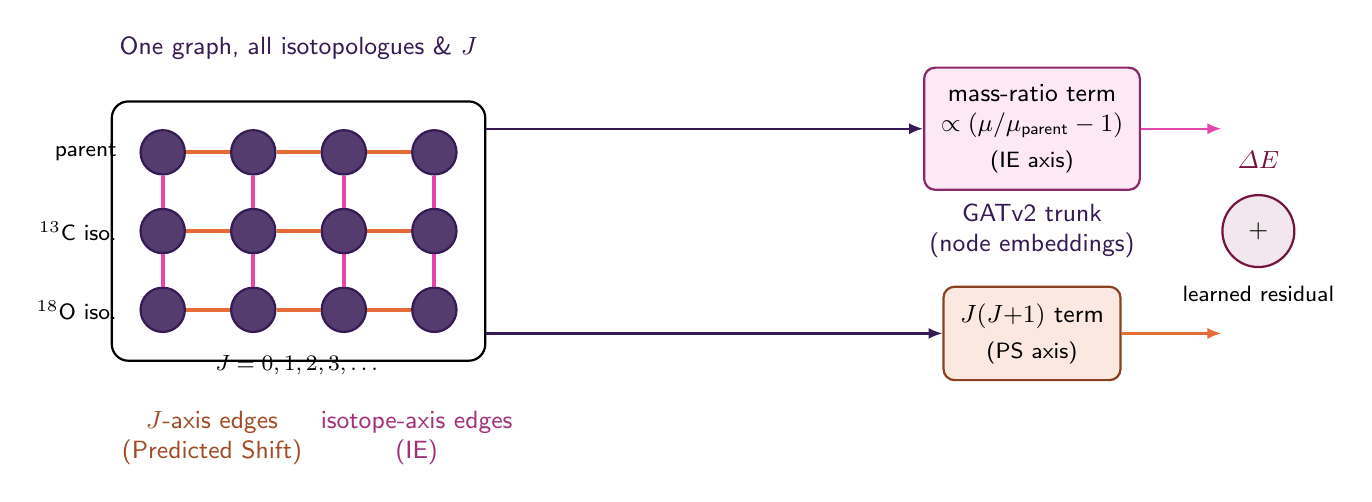
\begin{tikzpicture}[x=1.15cm,y=1.0cm]

  % --- GRAPH GRID: rows = isotopologues (isotope axis), columns = J (J axis) ---
  \foreach \row/\name in {0/parent,1/^{13}\text{C},2/^{18}\text{O}}{
    \foreach \col in {0,1,2,3}{
      \node[level] (N-\row-\col) at (\col,-\row) {};
    }
  }

  % J-axis edges (within an isotopologue, across J) — Predicted Shift axis
  \foreach \row in {0,1,2}{
    \foreach \col [count=\nextcol from 1] in {0,1,2}{
      \draw[j edge] (N-\row-\col) -- (N-\row-\nextcol);
    }
  }

  % Isotope-axis edges (same J, across isotopologues) — IE axis
  \foreach \col in {0,1,2,3}{
    \draw[iso edge] (N-0-\col) -- (N-1-\col);
    \draw[iso edge] (N-1-\col) -- (N-2-\col);
  }

  % Row labels (isotopologues)
  \node[axislabel, anchor=east] at (-0.4,0)  {parent};
  \node[axislabel, anchor=east] at (-0.4,-1) {$^{13}$C iso.};
  \node[axislabel, anchor=east] at (-0.4,-2) {$^{18}$O iso.};

  % Column label (J)
  \node[axislabel] at (1.5,-2.7) {$J = 0,1,2,3,\dots$};

  \begin{pgfonlayer}{background}
    \node[draw, thick, rounded corners=6pt, inner sep=10pt, fill opacity=0.05,
          fit=(N-0-0)(N-2-3)] (graphbox) {};
  \end{pgfonlayer}
  \node[label, uclDarkPurple, above=4mm of graphbox.north] {One graph, all isotopologues \& $J$};

  % Axis legend, below the graph box (out of the way of the arrows to the right)
  \node[label, uclLightOrange!70!black, below=5mm of graphbox.south, anchor=north, xshift=-1.1cm]
    {$J$-axis edges\\(Predicted Shift)};
  \node[label, uclLightPink!70!black, below=5mm of graphbox.south, anchor=north, xshift=1.5cm]
    {isotope-axis edges\\(IE)};

  % --- LINEAR PHYSICS BYPASS TERMS ---
  \node[term box iso] (massterm) at (9.6,0.3) {mass-ratio term\\$\propto (\mu/\mu_{\text{parent}} - 1)$\\[2pt]\footnotesize(IE axis)};
  \node[term box j] (jterm) at (9.6,-2.3) {$J(J{+}1)$ term\\[2pt]\footnotesize(PS axis)};
  \node[label, uclDarkPurple] at (9.6,-1.0) {GATv2 trunk\\(node embeddings)};

  \node[sum node] (sum) at (12.1,-1.0) {$+$};
  \node[label, uclDarkRed, above=2mm of sum] {$\varDelta E$};
  \node[axislabel, below=1mm of sum] {learned residual};

  \draw[thick,uclLightPink,-{Latex[length=5,width=4]}] (massterm.east) -- (sum.west |- massterm);
  \draw[thick,uclLightOrange,-{Latex[length=5,width=4]}] (jterm.east) -- (sum.west |- jterm);
  \draw[thick,uclDarkPurple,-{Latex[length=5,width=4]}] (graphbox.east |- massterm) -- (massterm.west);
  \draw[thick,uclDarkPurple,-{Latex[length=5,width=4]}] (graphbox.east |- jterm) -- (jterm.west);

\end{tikzpicture}
\end{document}
